\chapter{Introduction}

\begin{goals}
\item Understand the basic history of computer science
\item Know the components of a computer
\item Understand the different types of computers
\item Consider careers in computer science
\end{goals}

\section{Brief history of computer science}

The history of inventions is complicated, so assigning faces and dates to specific technologies that are often many years and people in the making is difficult. For an excellent layman's survey of the history of computer science, check out ``The Innovators" by Walter Isaacson. To give a general sense of where / when advancements were made, though, here is a brief summary: 

Timeline:
\begin{itemize}
\item Design of first modern-style computer + conceptualization of promise of computers (Charles Babbage and Ada the Countess of Lovelace, England, 1830-40)
\item Invention of the first electronic, programmable, general-purpose computer ``ENIAC" (John Mauchly and Presper Eckert, Pennsylvania, 1945)
\item Invention of the transistor (John Bardeen and Walter Brattain, New Jersey, 1947)
\item Invention of the first computer network (early Internet) ``ARPANET" (Bob Taylor and Larry Roberts, across the US, 1960s - 1970s)
\item First program that can run on a home hobbyist computer (Bill Gates and Paul Allen, New Mexico, 1975)
\item First simple and integrated computer for the common man ``Apple II" (Steve Jobs and Steve Wozniak, California, 1977)
\item Invention of the World Wide Web (Sir Tim Berners-Lee, Switzerland, 1990)
\end{itemize}

\begin{figure}
	\centering
	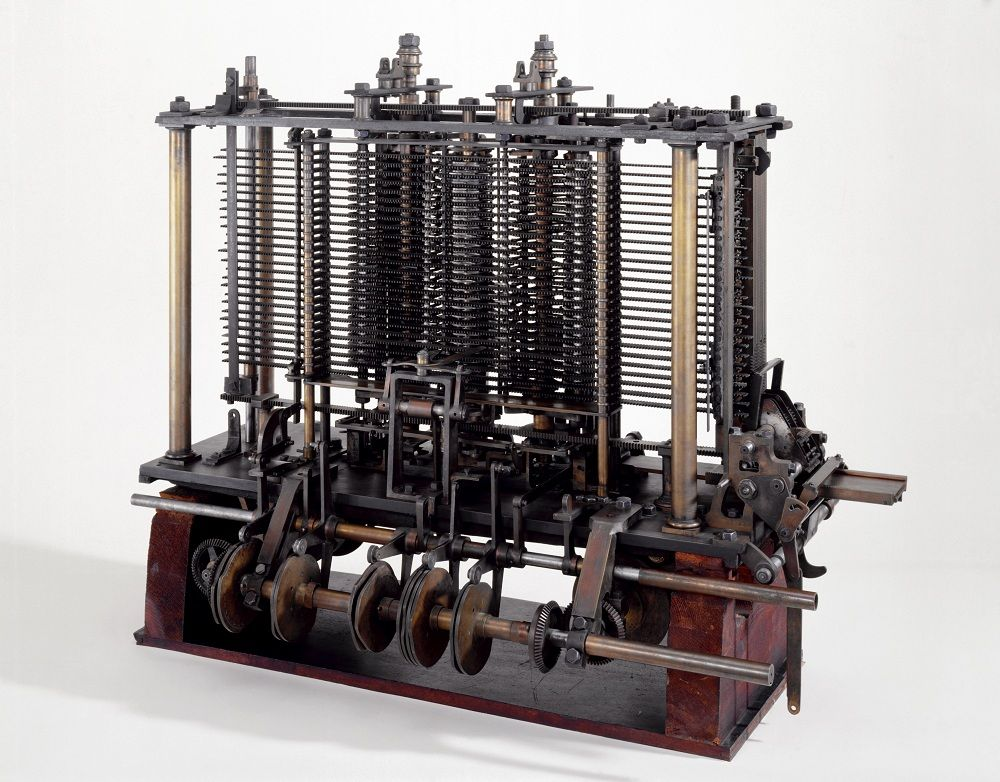
\includegraphics[width=0.85\textwidth]{images/analytic_engine.jpg}
	\caption{Charles Babbage's Victorian-era computer, called the ``Analytical Engine". Ada Lovelace worked closely with Babbage and was inspired to imagine how powerful future computers would be. 
    https://www.livescience.com/20718-computer-history.html}
	\label{fig:analytic_engine}
\end{figure}

\section{Components of a computer}

There are 4 primary components of a computer:

\begin{itemize}
	\item Hardware
	\item Software
	\item Data
	\item User
\end{itemize}

\subsection{Hardware}

Computer hardware consists of physical, electronic devices. These are the parts you actually can see and touch. Some examples include

\begin{itemize}
	\item Central processing unit (CPU)
	\item Monitor
	\item CD drive
	\item Keyboard
	\item Computer data storage
	\item Graphic card
	\item Sound card
	\item Speakers
	\item Motherboard
\end{itemize}

\begin{figure}
	\centering
	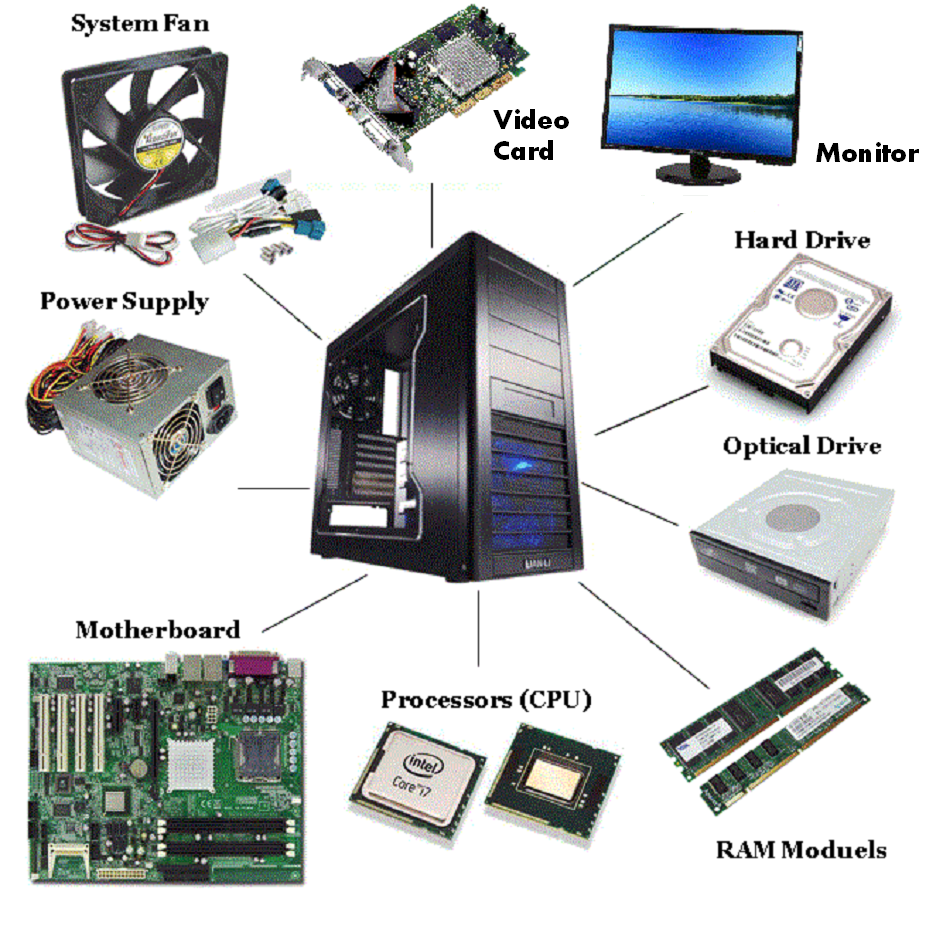
\includegraphics[width=0.85\textwidth]{images/hardware.png}
	\caption{Examples of hardware components of a personal computer. https://www5.cob.ilstu.edu/dsmath1/tag/computer-hardware/}
	\label{fig:hardware}
\end{figure}

We will discuss these components in more detail in a later lecture. 

\subsection{Software}

Software (otherwise known as \textit{programs}, \textit{applications}, or \textit{apps}) are organized sets of instructions for controlling the computer.

There are two main classes of software:

\begin{itemize}
	\item Applications software: programs allowing the human to interact directly with the computer
	\item Systems software: programs the computer uses to control itself
\end{itemize}

Some more familiar applications software include:

\begin{itemize}
	\item Microsoft Word: allows the user to edit text files
	\item Internet Explorer: connects the user to the world wide web
	\item iTunes: organizes and plays music files
\end{itemize}

While applications software allows the user to interact with the computer, systems software keeps the computer running. The operating system (OS) is the most common example of systems software, and it schedules tasks and manages storage of data.

We will dive deeper into the details of both applications and systems software in lecture 4.

\subsection{Data}
Data is fundamentally information of any kind. One key benefit of computers is their ability to reliably store massive quantities of data for a long time. Another is the speed with which they can do calculations on data once they receive instructions from a human user.

While humans can understand data with a wide variety of perceptions (taste,
smell, hearing, touch, sight), computers read and write everything internally as
\textit{bits}, sequences of 0s and 1s.

Computers have software and hardware which allow them to convert their internal 0s and 1s into text, numerals, and images displayed on the monitor; and sounds which can be played through the speaker.

Similarly, computers have hardware and software that convert information from
the real world into bits: a microphone converts sound, a camera converts pictures, and a text editor converts character symbols.

\subsection{Users}
Of course, there would be no data and no meaningful calculations without the human user. Computers are ultimately tools for making humans more powerful.

As we will see in the next section, however, different types of computers have different roles for the user.


\section{Types of computers}

\subsection{Supercomputers}
These are the most powerful computers out there. They are used for problems that take along time to calculate. They are rare because of their size and expense, and therefore primarily used by big organizations like universities, corporations, and the government.

The user of a supercomputer typically gives the computer a list of instructions, and allows the supercomputer to run on its own over the course of hours or days to complete its task.

\begin{figure}
	\centering
	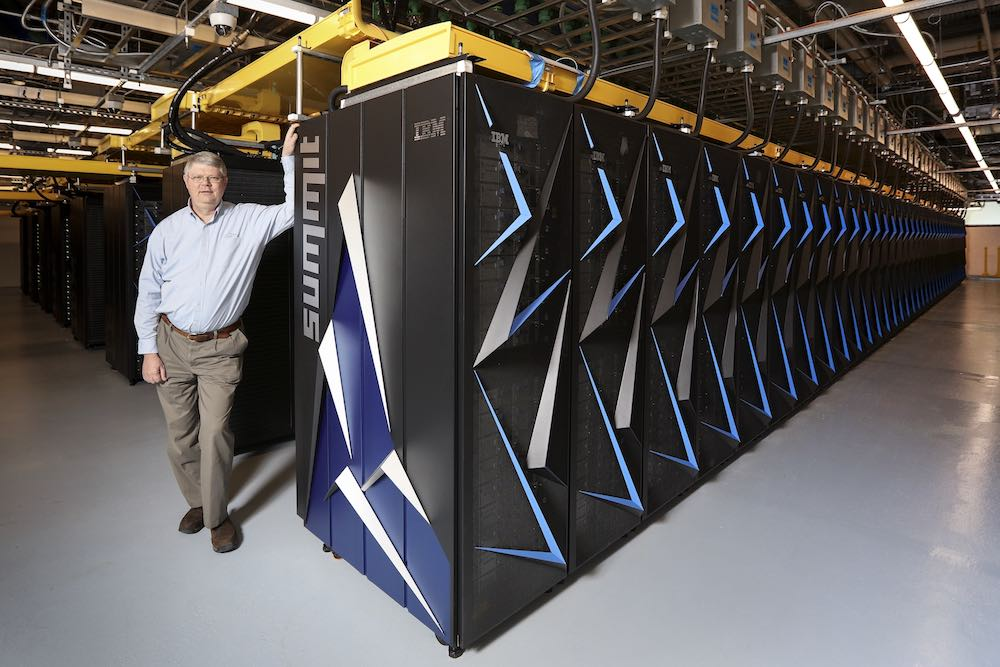
\includegraphics[width=0.85\textwidth]{images/supercomputer.jpg}
	\caption{Summit, a world-class supercomputing cluster at Oak Ridge National Laboratory in Tennessee. https://insidehpc.com/2018/11/new-top500-list-lead-doe-supercomputers/}
	\label{fig:supercomputer}
\end{figure}

\subsection{Mainframe computers}
Although not as powerful as supercomputers, mainframe computers can handle more data and run much faster than a typical personal computer. Often, they are given instructions only periodically by computer programmers, and then run on their own for months at a time to store and process incoming data. For example, census number-crunching, consumer statistics, and transactions processing all use mainframe computers.

\subsection{Personal computers}
These are the familiar computers we use to interact with applications every day. Full-size desktop computers and laptop computers are examples.

\subsection{Embedded computers}
In the modern ``digital'' age, nearly all devices we use have computers embedded within them. From cars to washing machines to watches to heating systems, most everyday appliances have a computer within them that allows them to function.

\subsection{Mobile computers}
In the past 2 decades, mobile devices have exploded onto the scene, and smartphones have essentially become as capable as standalone personal computers for many tasks.

\section{Why computers are useful}

Computers help us in most tasks in the modern age to make our lives easier and more comfortable. They are able to complete these tasks quickly and simultaneously. We can use them, for example, to:

\begin{itemize}
	\item Write a letter.
	\item Do our taxes.
	\item Play video games.
	\item Watch videos.
	\item Surf the internet.
	\item Keep in touch with friends.
	\item Date.
	\item Order food.
	\item Control robots and self-driving cars.
\end{itemize}

Computer technologies are at the core of many endeavors to make meaningful differences in the world, whether through space exploration, medical advances, expanding communication, or furthering education. As the digital age rises and computers become more embedded into our daily lives, it is increasingly important for everyone to understand how computers work, and how to use them. The job market for computer scientists is continuing to expand, and Computer skills are more and more necessary even in non-computational jobs.

According to a Stack Overflow survey from 2018,\footnote{https://insights.stackoverflow.com/survey/2018/} 9\% of professional coders on the online developer community have only been coding for 0-2 years. This demonstrates two things:

\begin{enumerate}
	\item The job market for people with coding skills is continually expanding
	\item It doesn't take much to become a coder
\end{enumerate}

Some examples of careers in computer science include:

\begin{itemize}
\item Information Technology (IT) manager/consultant: analyzes the technology needs of organizations and make computer systems recommendations. (Base Salary: \$85,000 - \$90,000)
\item Game developer: programs and develops console, computer, and mobile video-games from concept to actual product. (Base Salary: \$52,000 - \$127,000)
\item Web developer: takes a web design and turns it into a website by writing lines of code in a variety of programming languages. (Base Salary: \$52,000 - \$110,000)
\item UI/UX designer: UI stands for “user interface” and UX stands for “user experience.” UI designers focus on the look and layout of a product. UX designers focus on how a product works and how people interact with it. (Base Salary: \$59,000 - \$110,000)
\item Data analyst: retrieves and organizes data to reach meaningful conclusions with statistical, coding, and analytical tools. (Base Salary: \$45,000 - \$95,000)
\item Database manager: oversees an organization's data storage and retrieval system. (Base Salary: \$39,000 - \$87,000)
\end{itemize}
In this course, you will learn how to program a computer -- that is, how to instruct the computer to perform tasks. The concepts and skills you learn in this course will form an important foundation that will make you a more informed citizen, and perhaps, a computing professional. 

\exercisesection

\begin{figure}
  \centering
    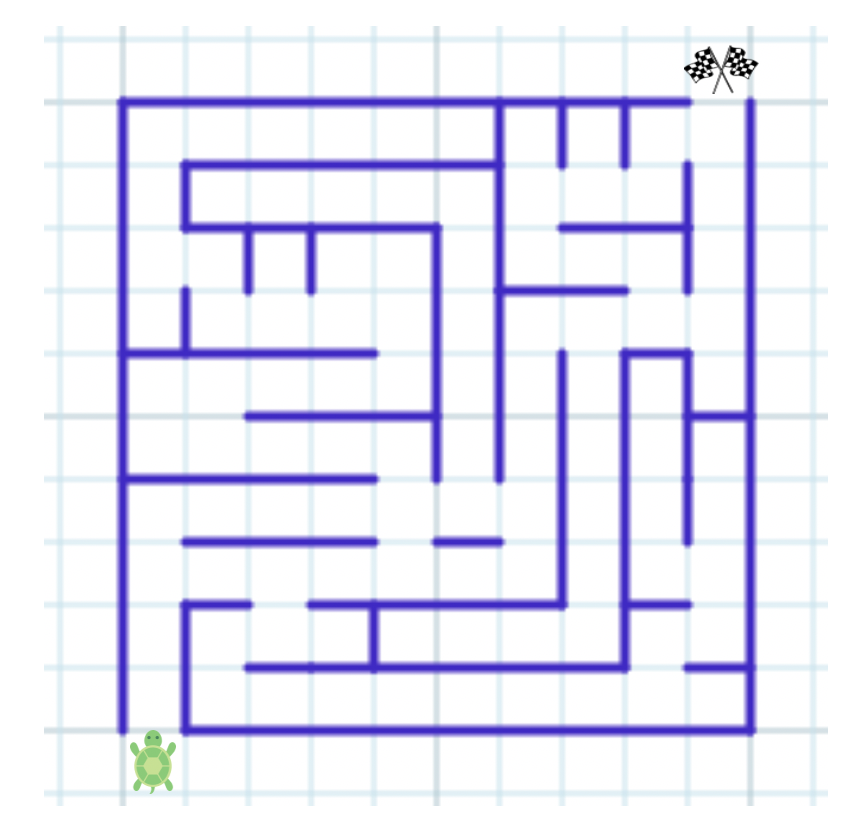
\includegraphics[width=.32\textwidth]{images/maze_example}
    %\includegraphics{maze2.png}
   % \includegraphics{maze3.png}
    \caption{An example maze. The roboturt starts at the box in the bottom left facing toward the top of the page. We need to get it to the box with the finish flags at the top right.}
    \label{fig:graph-paper}
\end{figure}

\begin{exercise}

For this exercise you are going to program a robotic turtle ("roboturt") to complete a maze. The roboturt accepts two commands:  ``Turn Left [number]'' (TL[n]) and ``Move Forwards [number]'' (MF[n]). TL tells the roboturt to change the direction it's facing without moving out of its box (and note that 3 lefts can make a right). MF tells the roboturt to step into the box in front of it. For example, the following commands would tell the roboturt to complete the example maze shown in Figure ~\ref{fig:graph-paper}.: MF[4], TL[3], MF[6], TL[1], MF[3], TL[3], MF[3], TL[1], MF[4]. A visual representation of the roboturt following these commands is in Figure~\ref{fig:turtle_sequence}.

  Get a piece of graph paper, and build your own maze on it. Make sure to draw a roboturt in the starting box in whatever direction you want it to start in, and a flag at the finish box. You may refer to the maze on Figure~\ref{fig:graph-paper}as an example. 
  
First create a list of commands that tells the robot to complete your own maze. Then do the same for another student's maze. Compare your command sequences. 

  What types of commands could have made this easier? Could your robot solve
  arbitrary mazes? What types of commands would be helpful for making your robot
  solve any maze?
\end{exercise}


\begin{figure}
  \centering
    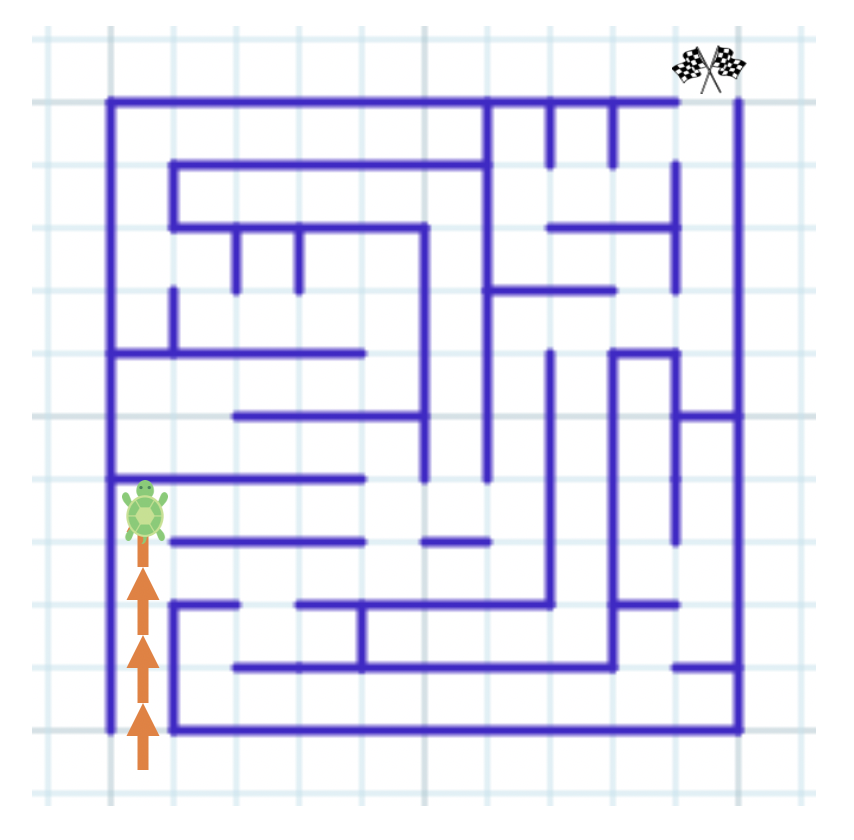
\includegraphics[width=.32\textwidth]{images/turtle_1}
    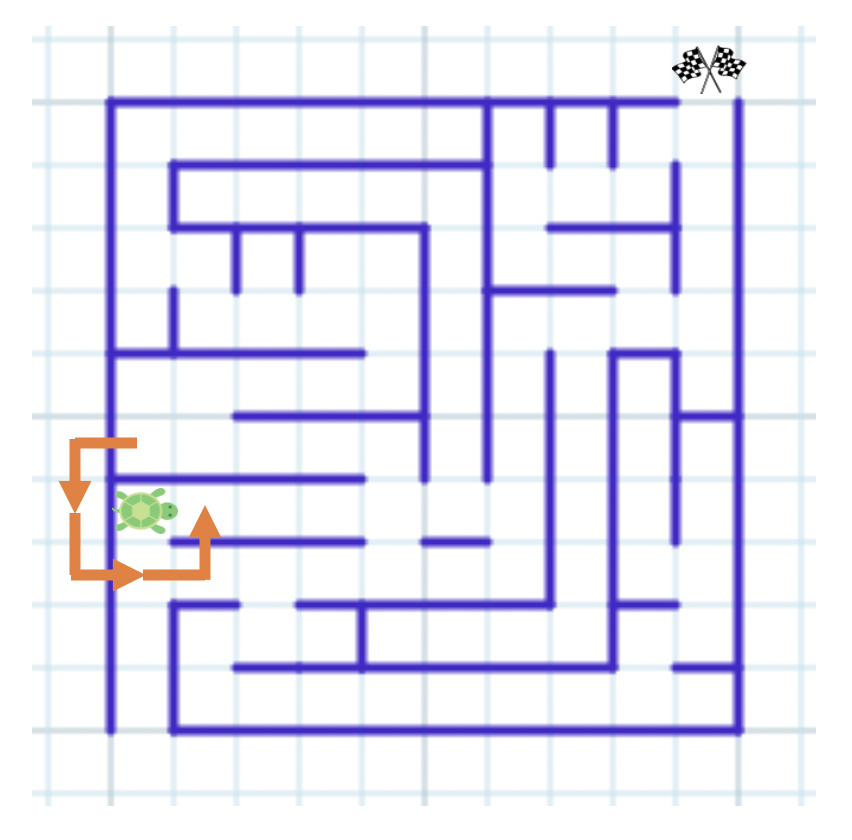
\includegraphics[width=.32\textwidth]{images/turtle_2}
    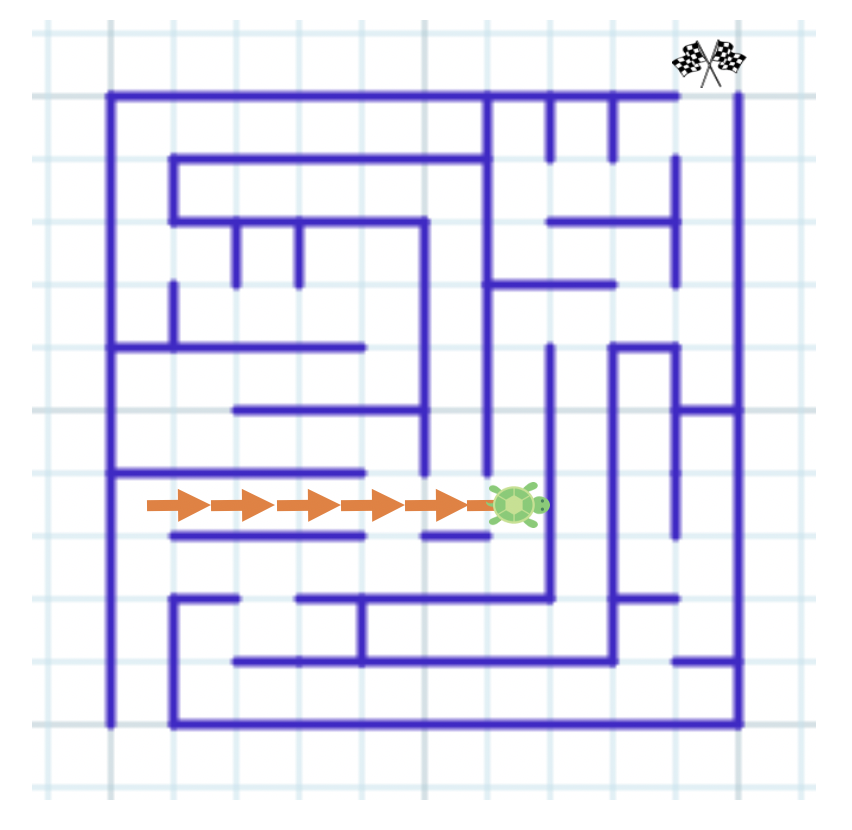
\includegraphics[width=.32\textwidth]{images/turtle_3}
    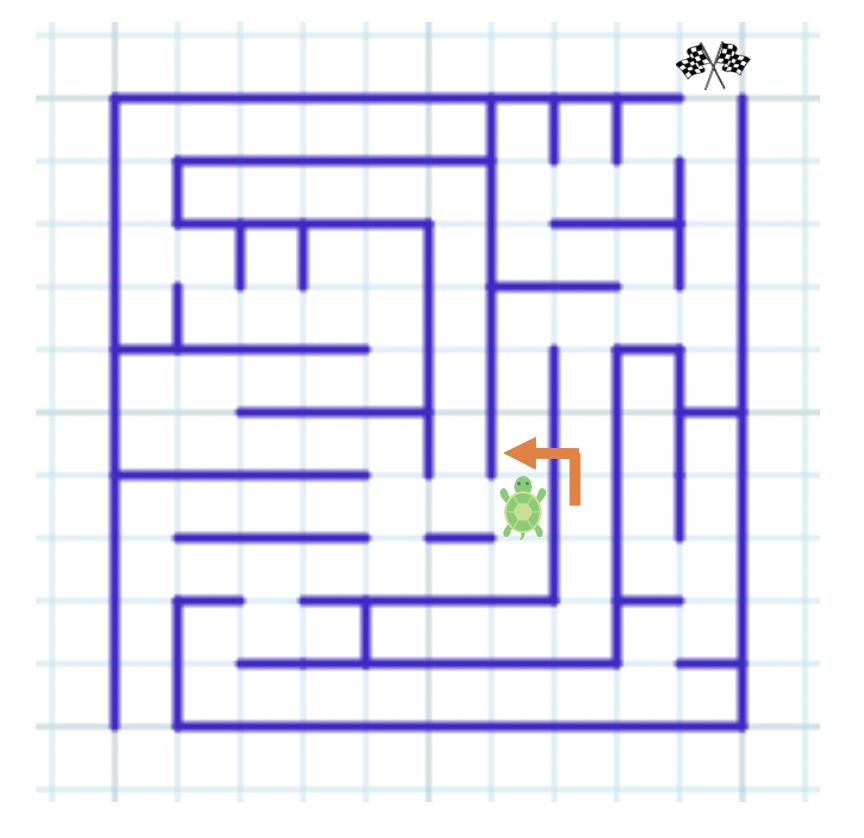
\includegraphics[width=.32\textwidth]{images/turtle_4}
    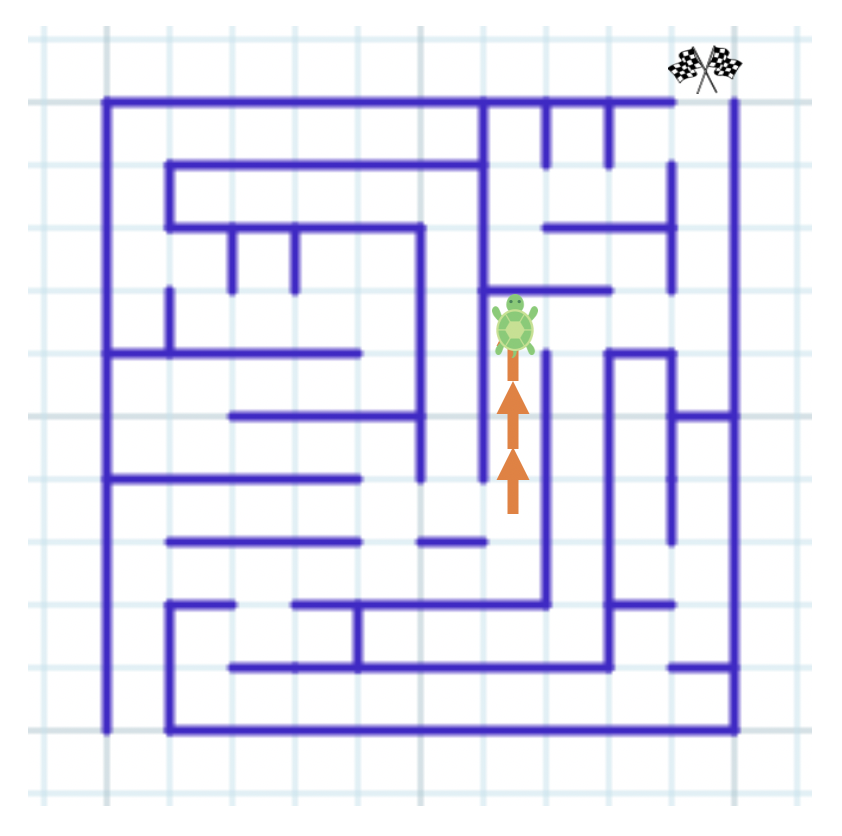
\includegraphics[width=.32\textwidth]{images/turtle_5}
    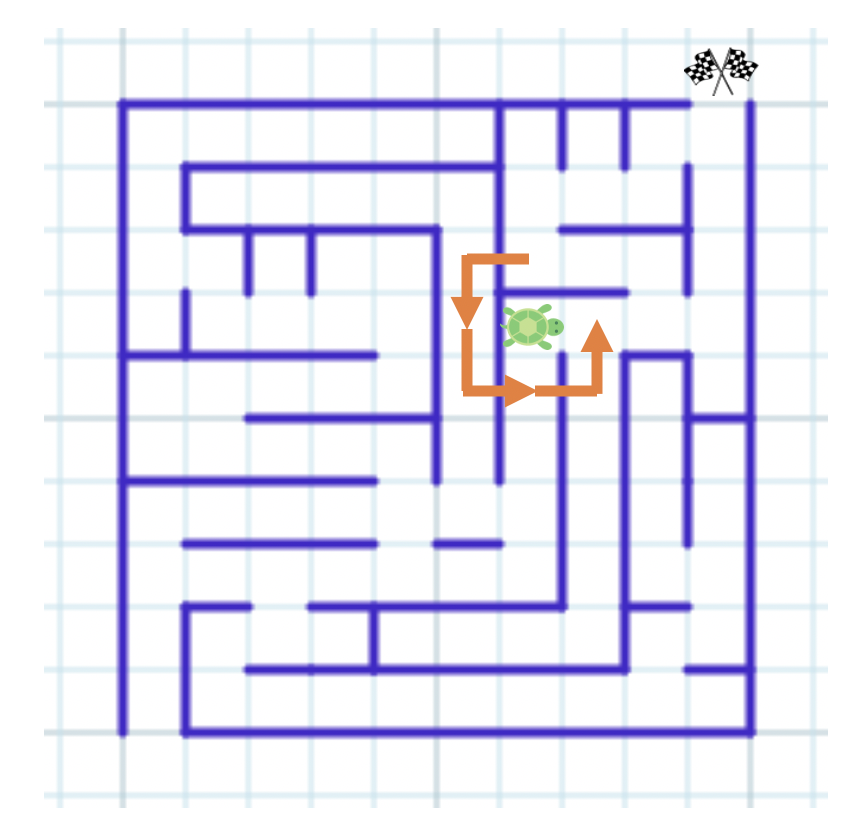
\includegraphics[width=.32\textwidth]{images/turtle_6}
    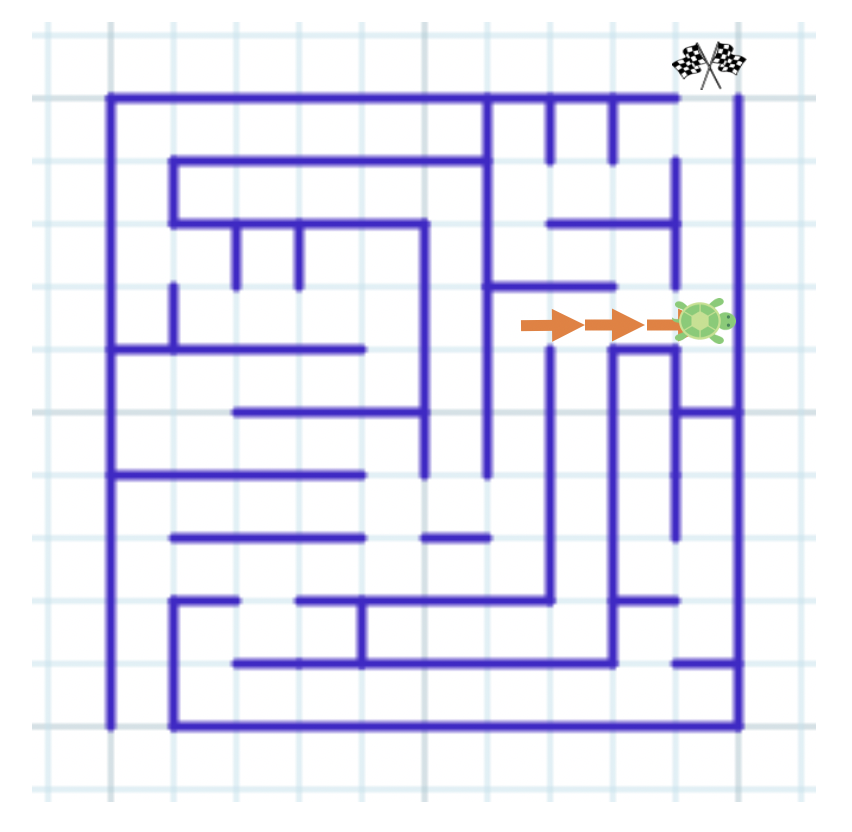
\includegraphics[width=.32\textwidth]{images/turtle_7}
    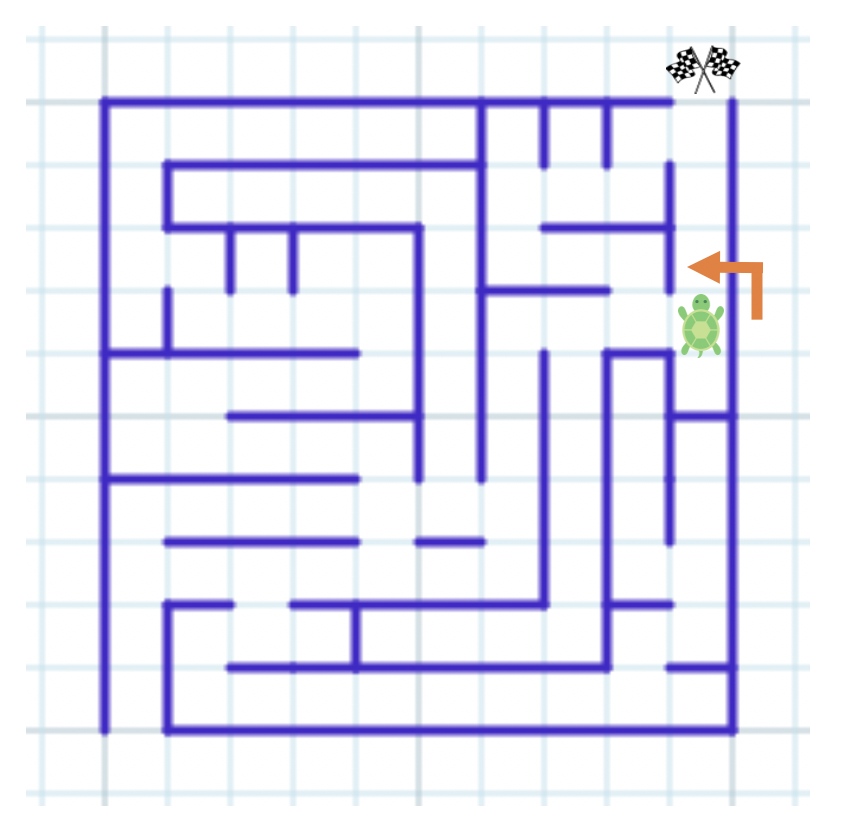
\includegraphics[width=.32\textwidth]{images/turtle_8}
    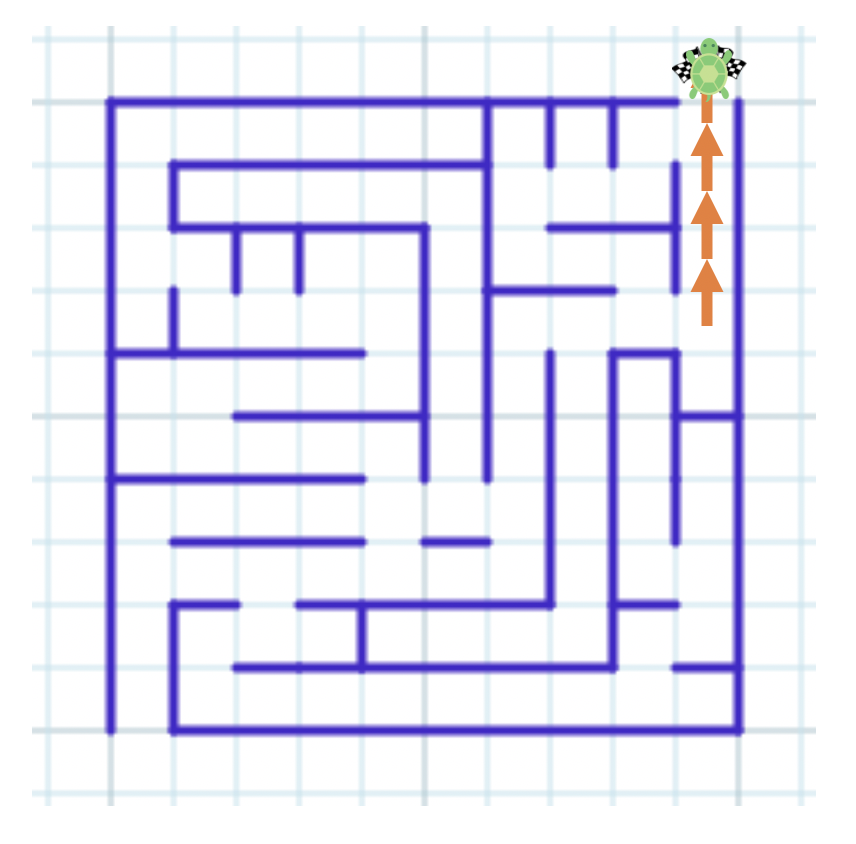
\includegraphics[width=.32\textwidth]{images/turtle_9}
    %\includegraphics{maze2.png}
   % \includegraphics{maze3.png}
    \caption{A visual representation of what happens when the roboturt follows the commands (MF[4], TL[3], MF[6], TL[1], MF[3], TL[3], MF[3], TL[1], MF[4]).}
    \label{fig:turtle_sequence}
\end{figure}

\begin{exercise}
What are some other tasks a computer can accomplish?
\end{exercise}

\begin{exercise}
  Think about building a simple video game. What are the hardware, software, and
  data needed for this game? What would be the minimal hardware, and what
  hardware would you need to add features like voice chat or online play? What
  types of computers would best run this game? Why?

  Do the same for a text editor and an ATM machine. 
\end{exercise}


\referencessection

\textit{Computer Science: An Interdisciplinary Approach}, Robert Sedgewick and Kevin Wayne.

University of Wisconsin-Madison CS 202 Lectures, Andrea Arpaci-Dusseau.\\http://pages.cs.wisc.edu/~dusseau/Classes/CS202-F11/
